\Chapter{Proposed Method}\label{chapter:proposed-method}

In this chapter, I describe the proposed method for adapting a pre-trained 2D diffusion model to understand 3D geometry and synthesize novel views of objects. The approach focuses on conditioning the generative process on both a reference image and relative camera transformations.

\section{Research Motivation and Gaps}\label{sec:limitations}

Despite the significant progress in diffusion-based novel view synthesis, several critical limitations motivate the development of my approach:

\begin{enumerate}
  \item \textbf{Training Efficiency vs. Model Expressiveness}: While MV-Adapter \cite{mvadapter} introduced adapter-based training for multi-view generation, existing approaches face a trade-off between computational efficiency and model expressiveness. Full fine-tuning provides maximum flexibility but is computationally prohibitive for large models, while extremely lightweight adapters may limit the model's ability to learn complex 3D relationships.

  \item \textbf{Camera Conditioning Limitations}: Current methods predominantly rely on either simple pose vectors (Zero-1-to-3 \cite{zero1to3}) or complex raymap representations (CAT3D \cite{cat3d}, MV-Adapter \cite{mvadapter}). Pose vectors provide insufficient geometric detail for complex viewpoint changes, raymaps inherently struggle to model complex materials like glass or reflective surfaces, and often introduce visual artifacts that disrupt the diffusion model's ability to synthesize realistic images.

  \item \textbf{Feature Integration Strategies}: Most existing methods either use cross-attention for all conditioning (requiring significant architectural modifications) or global feature concatenation (limiting spatial awareness). There is a gap in exploring hybrid conditioning strategies that can leverage both global geometric understanding and detailed visual feature transfer.

  \item \textbf{Training Data Quality and Lighting Inconsistencies}: A critical limitation affecting novel view synthesis quality stems from inconsistent lighting conditions in training data. The standard Objaverse rendering pipeline employs randomized lighting setups which, while intended to introduce variability, often result in images with harsh lighting, strong shadows, or scenes where objects are underexposed or completely obscured due to unfavorably positioned light sources. This inconsistency severely impacts the model's ability to learn reliable appearance and geometric relationships, directly affecting downstream 3D reconstruction applications where view consistency is crucial. The next chapter (Chapter \ref{chapter:data-preparation}) details the data preparation approach that addresses this issue.

  \item \textbf{Limited Viewpoint Generalization}: Existing methods trained on specific sets of camera perspectives often fail to generalize to novel viewpoint configurations. This constraint limits their effectiveness for applications requiring flexible camera positioning and novel view synthesis from arbitrary viewpoints.

  \item \textbf{Adaptation to Unseen Objects}: Current methods often struggle to generalize beyond the object categories and styles present in their training data. This limitation becomes particularly apparent when applying trained models to real-world objects with different materials, textures, or geometric properties than those encountered during training, limiting practical applicability.

\end{enumerate}

\textbf{My Contributions}: This work addresses these limitations through: (1) a balanced adapter architecture that maintains expressiveness while ensuring training efficiency, (2) a FiLM-based camera conditioning mechanism that enables direct geometric control through learnable camera parameter encoding, (3) a hybrid conditioning strategy combining parallel image cross-attention with network modulation, (4) carefully curated training data with consistent lighting conditions, (5) training on diverse viewpoint configurations as well as (6) diverse object categories to maximize generalization capabilities.

\section{Theoretical Justification}\label{sec:theoretical-justification}

The core innovation of this work lies in the application of Feature-wise Linear Modulation (FiLM) for camera parameter conditioning in diffusion models. This section provides theoretical justification for why this approach is fundamentally well-suited for novel view synthesis.

\subsection{Geometric Transformations and Feature Space Modulation}

Camera transformations between viewpoints can be decomposed into rotation matrix $\mathbf{R} \in SO(3)$ and translation vector $\mathbf{t} \in \mathbb{R}^3$, which define how 3D points transform between coordinate systems. In the context of novel view synthesis, we seek to transform feature representations from a source viewpoint to a target viewpoint.

The key insight is that FiLM's affine transformation $\gamma \odot \mathbf{h} + \beta$ provides a learnable approximation of geometric transformations in feature space. Specifically:

\begin{itemize}
  \item \textbf{Scaling component} ($\gamma$): Can model perspective changes, depth-dependent scaling, and orientation-dependent feature emphasis that arise from rotational transformations
  \item \textbf{Shift component} ($\beta$): Can model translational offsets and view-dependent bias adjustments needed to account for position changes
\end{itemize}

\subsection{Cross-Modal Conditioning}

FiLM has been proven effective for cross-modal conditioning, where information from one modality (e.g., text) influences processing in another modality (e.g., images) \cite{film, filmedunet}. Our application extends this framework by treating camera parameters as a distinct geometric modality.

The theoretical foundation rests on FiLM's ability to perform \textit{conditional computation} - the same feature map $\mathbf{h}$ can be processed differently based on the conditioning signal. For camera conditioning:

\[ \text{FiLM}(\mathbf{h}|\mathbf{R}, \mathbf{t}) = \gamma(\mathbf{R}, \mathbf{t}) \odot \mathbf{h} + \beta(\mathbf{R}, \mathbf{t}) \]

where $\gamma$ and $\beta$ are learned functions of the camera parameters. This formulation allows the network to dynamically adjust its feature processing based on the target viewpoint, effectively implementing view-dependent feature transformations.

\subsection{Hybrid Conditioning Strategy}

The combination of FiLM-based camera conditioning with parallel image cross-attention is motivated by the complementary nature of these mechanisms:

\begin{itemize}
  \item \textbf{FiLM conditioning}: Provides global, view-dependent modulation that affects how features are processed throughout the network
  \item \textbf{Image cross-attention}: Enables selective attention to relevant visual details from the reference image
\end{itemize}

This hybrid approach allows the model to both globally adapt its processing for the target viewpoint (via FiLM) and selectively transfer appropriate visual content (via attention), addressing the fundamental challenge of novel view synthesis: maintaining visual consistency while adapting to geometric changes.

\section{Method Overview}\label{sec:overview}

\subsection{Method Summary}
My proposed method adapts Stable Diffusion 2.1 for multi-view novel view synthesis by introducing two specialized conditioning streams. The method leverages strong generative capabilities of the pre-trained 2D diffusion model while equipping it with 3D spatial understanding through minimal architectural modifications.

\begin{figure}[htbp]
  \centering
  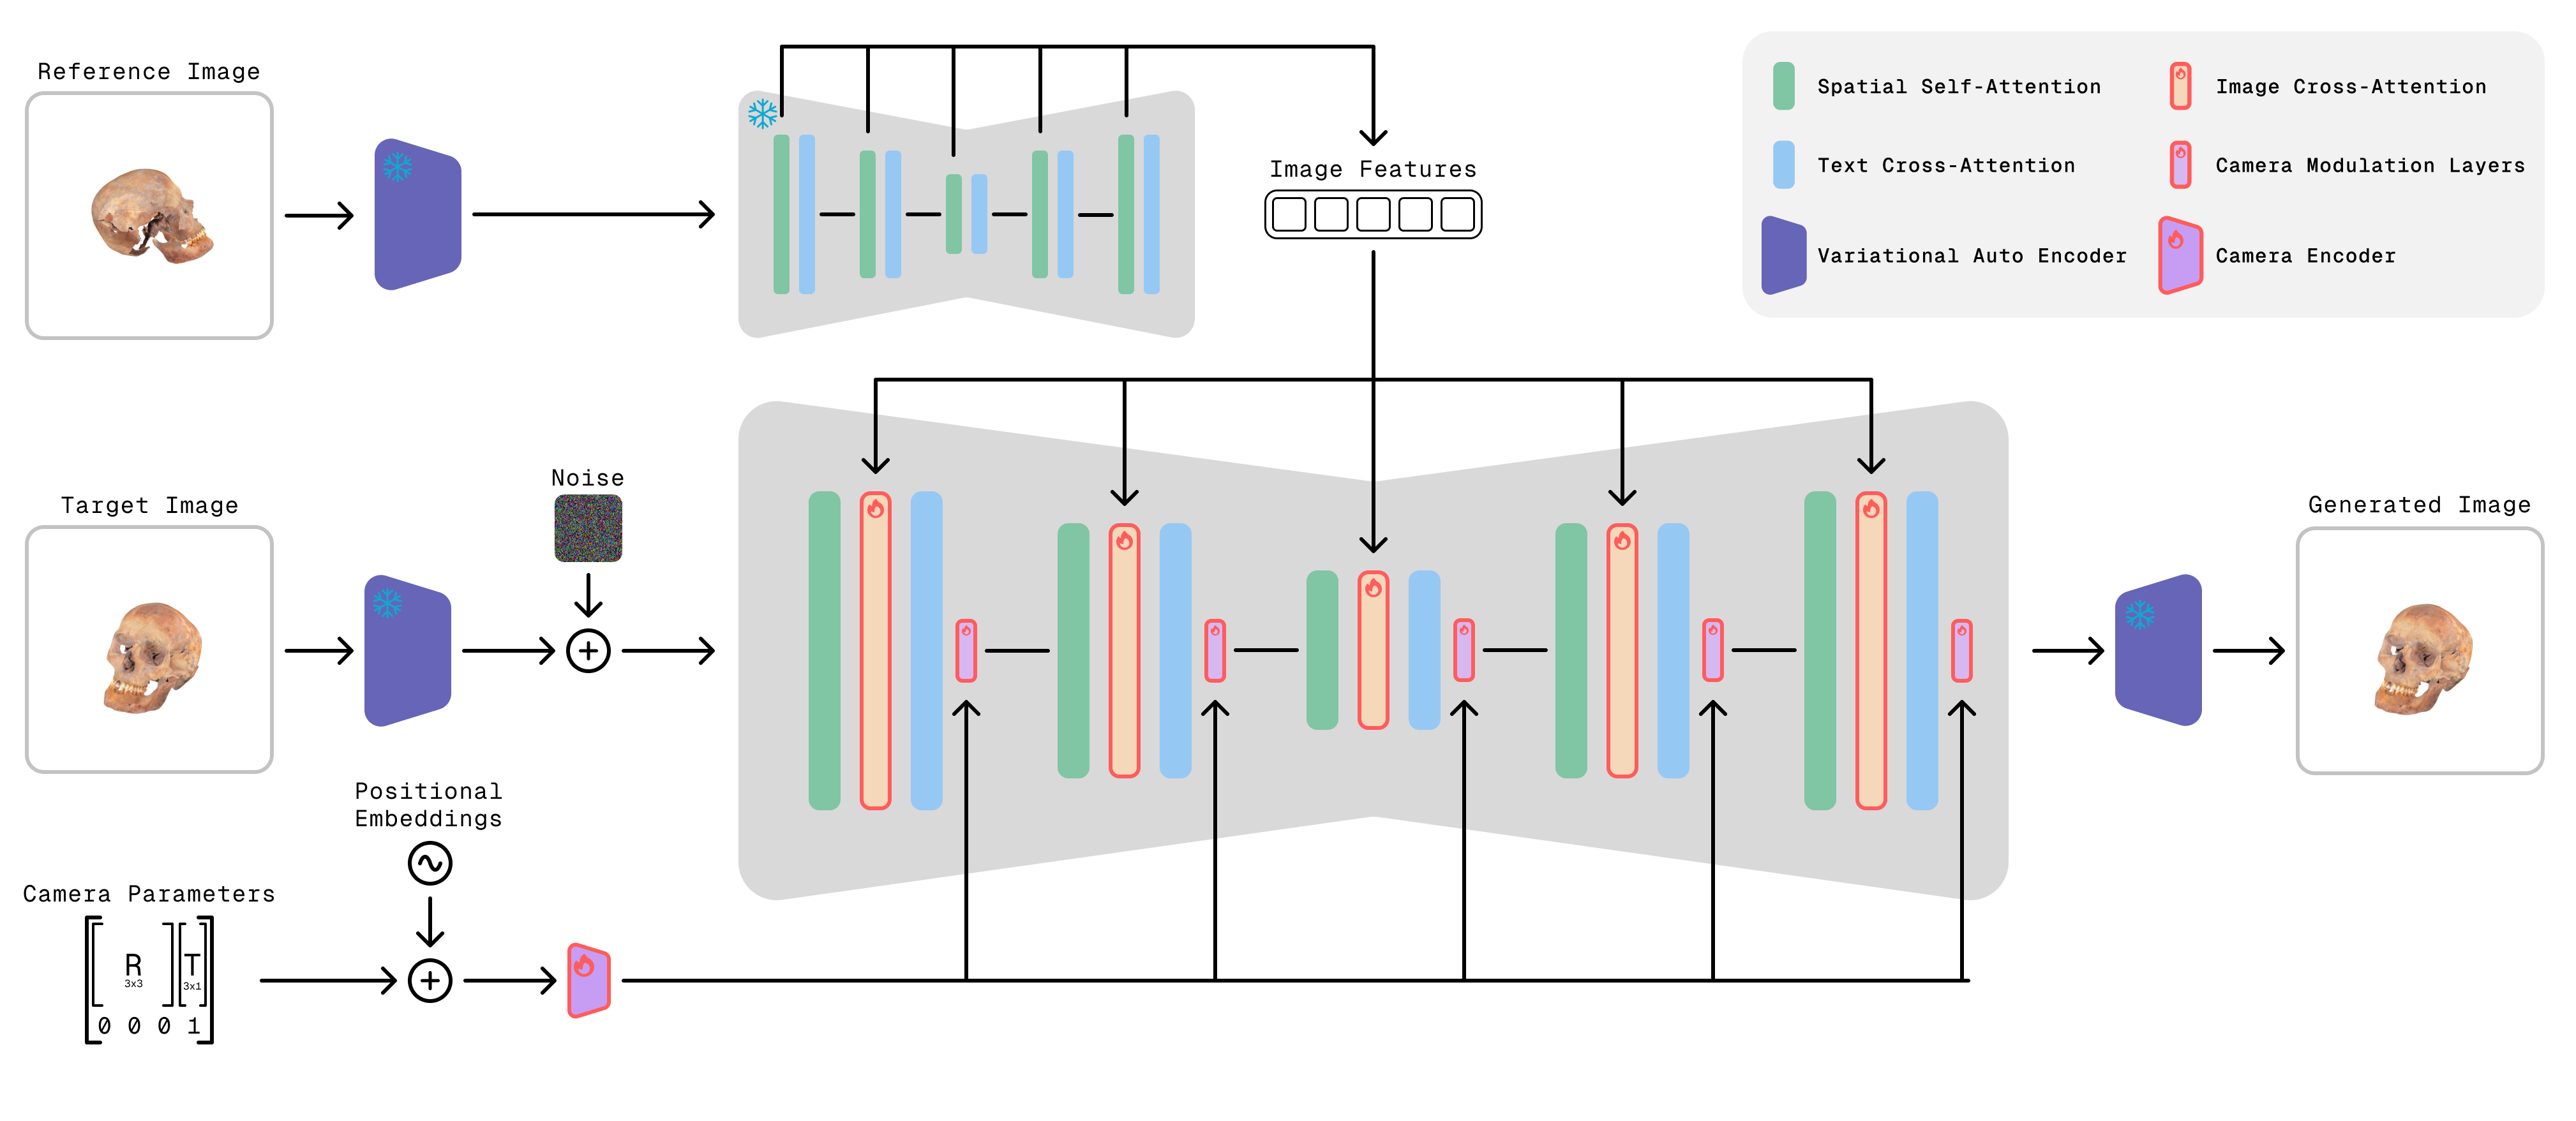
\includegraphics[width=\textwidth]{images/proposed-method/my-method-diagram.png}
  \caption{System diagram of the proposed multi-view diffusion model. It showcases the reference image encoding path, the camera parameter encoding path, and their integration into the main denoising U-Net.}
  \label{fig:my-method-diagram}
\end{figure}

The method adapts the Stable Diffusion 2.1 model, an inherently 2D generative framework, to comprehend 3D spatial relationships and generate images from novel viewpoints. The system achieves this by integrating two distinct conditioning streams into the diffusion model's U-Net architecture. The first stream provides visual context from a source (reference) image, while the second stream imparts geometric awareness through encoded camera parameters.

Figure \ref{fig:my-method-diagram} illustrates the overall architecture of the proposed system, highlighting the flow of information and the interplay between the original diffusion model components and the newly introduced conditioning modules.

\subsection{Core Innovation}
The key innovation lies in the hybrid conditioning approach that combines:
\begin{itemize}
  \item \textbf{Visual conditioning}: Parallel image cross-attention adapters that preserve visual consistency
  \item \textbf{Geometric conditioning}: FiLM-based camera parameter modulation for spatial awareness
  \item \textbf{Efficiency}: Adapter-based training that keeps the backbone model frozen
\end{itemize}

\section{Architectural Framework}\label{sec:architectural-framework}
In my method I leverage the strong generative capabilities of a pre-trained 2D diffusion model and extend it for 3D-aware novel view synthesis. This is achieved through the introduction of specialized conditioning modules that inject visual and geometric information into the denoising U-Net.

\subsection{Backbone: Stable Diffusion 2.1}
The foundation of the proposed method is the Stable Diffusion 2.1 model. I chose this model for its robust text-to-image generation capabilities, clear architectural design, and its publicly available pre-trained weights, which encapsulate extensive understanding of visual concepts. The core component relevant to my modifications is its U-Net architecture \cite{unet}, which performs the iterative denoising process.

In my method I keep several key components of the original model frozen to preserve their learned knowledge and ensure computational efficiency during training. These include the Variational Autoencoder (VAE) \cite{vae} used for encoding images into and decoding latents from the latent space, the text encoder CLIP \cite{clip} responsible for processing textual prompts, and the weights of the original U-Net when used within the Reference Image Encoder. I specifically designed the new conditioning modules and adapters to be trainable while maintaining the frozen backbone.

\subsection{Reference Image Conditioning Stream}
To enable the model to generate views that are visually consistent with a given input, a reference image conditioning stream is introduced. This approach is inspired by recent advances in image-conditioned generation, particularly the feature extraction strategies employed in CatVTON \cite{catvton} for garment transfer and the multi-view attention mechanisms developed in MV-Adapter \cite{mvadapter}. This stream aims to capture and transfer the appearance, texture, color, and identity of the object depicted in the source image to the novel view generation process.

\subsubsection{Source Image Feature Extraction}
The process of extracting visual features from the source image through a dedicated $\text{ImageEncoder}$ module leverages a frozen copy of the Stable Diffusion 2.1 U-Net to extract multi-scale attention features.

\textbf{Feature Extraction Process}: The method first encodes the source image into latent space using the VAE encoder. Then, the resulting latents are processed through a frozen copy of the Stable Diffusion 2.1 U-Net with timestep set to zero ($t=0$), effectively performing feature extraction (rather than denoising). During this forward pass, the $\text{ImageEncoder}$ registers forward hooks on attention layers throughout the U-Net architecture. This frozen U-Net copy is separate from the main denoising U-Net and serves purely for feature extraction, minimizing the number of trainable parameters. The hooks capture outputs from all the attention layers in the U-Net. These features encode visual information at different semantic levels, from low-level textures in early layers to high-level semantic concepts in deeper layers.

\subsubsection{Image Cross-Attention Adapters}
The visual features extracted by the $\text{ImageEncoder}$ are injected into the main denoising U-Net using newly introduced, trainable adapter modules that serve as cross-attention layers. These processors are designed to be lightweight and integrated into each corresponding block of the denoising U-Net.

\textbf{Parallel Architecture Design}: A key architectural choice is the parallel integration of these image cross-attention adapters, inspired by the adapter design philosophy of MV-Adapter \cite{mvadapter}. Instead of serially passing information through the original attention layers and then the new adapters, the adapters operate in parallel to the U-Net's existing self-attention and text-cross-attention mechanisms. This design choice preserves the original feature space while enabling efficient learning of image-conditioned representations, similar to the approach used in IP-Adapter \cite{ipadapter} for image prompt conditioning.

\textbf{Attention Mechanism}: The extracted image features serve as the key ($\mathbf{K}_{img}$) and value ($\mathbf{V}_{img}$) for these new cross-attention layers, while the U-Net's intermediate hidden states act as the query ($\mathbf{Q}$). The cross-attention operation is computed using scaled dot-product attention:
\[ \text{Attention}(\mathbf{Q}, \mathbf{K}_{img}, \mathbf{V}_{img}) = \text{softmax}\left(\frac{\mathbf{Q}\mathbf{K}_{img}^T}{\sqrt{d_k}}\right)\mathbf{V}_{img} \]

The output is scaled by a hyperparameter - reference scale factor and added to the original attention output:
\[ \mathbf{h}_{out} = \mathbf{h}_{original} + \text{ref\_scale\_val} \cdot \text{Attention}(\mathbf{Q}, \mathbf{K}_{img}, \mathbf{V}_{img}) \]

\textbf{Efficiency Considerations}: The adapter-based approach trains only 585M parameters out of the total 2.9B parameters of the complete model (including U-Net, VAE, text encoder, and adapters), ensuring computational efficiency while maintaining expressive power.

\subsection{Camera Parameter Conditioning Stream}
To ensure geometric consistency and enable precise control over the viewpoint of the generated image, the method employs a camera parameter conditioning stream. This stream encodes the relative transformation between the source and target camera poses and uses this information to modulate the behavior of the denoising U-Net.

\subsubsection{Camera Pose Encoding}
The $\text{CameraEncoder}$ module processes geometric information by computing and encoding the relative transformation between source and target camera poses.

\textbf{Relative Transformation Computation}: Following the relative pose encoding strategy established in Zero-1-to-3 \cite{zero1to3}, given source camera pose $\mathbf{C}_s$ and target camera pose $\mathbf{C}_t$ (both $4 \times 4$ homogeneous transformation matrices), the method first extracts rotation matrices $\mathbf{R}_s, \mathbf{R}_t \in \mathbb{R}^{3 \times 3}$ and translation vectors $\mathbf{t}_s, \mathbf{t}_t \in \mathbb{R}^3$. The relative transformation is computed as:
\[ \mathbf{R}_{rel} = \mathbf{R}_t \mathbf{R}_s^T \]
\[ \mathbf{t}_{rel} = \mathbf{t}_t - \mathbf{R}_{rel} \mathbf{t}_s \]

\textbf{Dual-Stream Encoding}: The method processes the relative rotation and translation through separate encoding streams.

Rotation Encoding: The $3 \times 3$ rotation matrix are flattened to a 9-dimensional vector and processed through a dedicated MLP:
\[ \mathbf{E}_{rot} = \text{MLP}_{rot}(\text{flatten}(\mathbf{R}_{rel})) \]

Translation Encoding: The translation vector $\mathbf{t}_{rel}$ is first positionally encoded to enrich its geometric representation, adapting the positional encoding technique from transformer architectures \cite{attention_is_all_you_need}:
\[ \text{PE}(\mathbf{t}_{rel}) = [\sin(\omega_k \cdot \mathbf{t}_{rel}), \cos(\omega_k \cdot \mathbf{t}_{rel})]_{k=1}^{K} \]
where $\omega_k = \exp(\frac{k \log(\omega_{max})}{K})$ are logarithmically spaced frequencies. The positionally encoded translation is then processed through its own MLP:
\[ \mathbf{E}_{trans} = \text{MLP}_{trans}(\text{PE}(\mathbf{t}_{rel})) \]

\textbf{Final Projection}: The rotation and translation embeddings are concatenated and projected to the final camera embedding dimension:
\[ \mathbf{E}_{cam} = \text{MLP}_{final}([\mathbf{E}_{rot}; \mathbf{E}_{trans}]) \]
where $\mathbf{E}_{cam} \in \mathbb{R}^{d_{cam}}$ represents the final camera embedding with dimension $d_{cam} = 2048$.

The MLP details are provided in the next chapter (Chapter \ref{chapter:experiments}).

\subsubsection{FiLM-based Network Modulation}
The high-dimensional camera embedding produced by the $\text{CameraEncoder}$ is used to modulate the activations within the main denoising U-Net via Feature-wise Linear Modulation (FiLM) layers \cite{film}. This approach is motivated by the success of FiLM in cross-modal conditioning tasks, particularly its application in FiLMed-UNet \cite{filmedunet} for medical image segmentation with metadata conditioning. As detailed in Chapter \ref{chapter:related}, FiLM provides an effective mechanism for conditioning neural network activations. Our novel contribution lies in applying this mechanism specifically to camera parameter conditioning in diffusion models, enabling camera pose information to dynamically influence feature representations throughout the network.

\textbf{Modulator Architecture}: For each U-Net block that requires camera conditioning, the method employs dedicated modulator networks that generate scale and shift parameters from the camera embedding:
\[ [\boldsymbol{\gamma}; \boldsymbol{\beta}] = \text{MLP}_{mod}(\mathbf{E}_{cam}) \]
where $\text{MLP}_{mod}$ is a two-layer MLP that maps the camera embedding to concatenated scale and shift parameters.

\textbf{FiLM Operation}: For a given feature map $\mathbf{h} \in \mathbb{R}^{B \times C \times H \times W}$ in the U-Net, the FiLM layer applies:
\[ \text{FiLM}(\mathbf{h}) = \boldsymbol{\gamma} \odot \mathbf{h} + \boldsymbol{\beta} \]
where $\boldsymbol{\gamma}, \boldsymbol{\beta} \in \mathbb{R}^C$ are channel-wise parameters, and $\odot$ denotes element-wise multiplication broadcast across spatial dimensions.

\textbf{Network Integration}: FiLM modulations are applied through forward hooks registered on the outputs of all the U-Net down-sampling blocks, middle block, and up-sampling blocks. The hooks intercept the block outputs and apply the corresponding camera-conditioned modulation before passing the features to subsequent layers.

\textbf{Initialization Strategy}: The modulator networks are initialized with small weights and biases set such that the initial scale parameters have mean 0.5 and shift parameters have mean 0.0. This ensures stable training initialization where the camera conditioning gradually integrates without disrupting pre-trained feature representations.

\subsection{The Integrated Conditioned U-Net}
The $\text{MultiViewUNet}$ module serves as the central component of the proposed architecture. It integrates the backbone Stable Diffusion U-Net with the two conditioning streams described above: the reference image conditioning via parallel Image Cross-Attention Adapters and the camera parameter conditioning via Feature-wise Linear Modulation (FiLM) layers.

During each step of the reverse diffusion process, the $\text{MultiViewUNet}$ takes the noisy latent representation of the target image, the current timestep, text embeddings, the extracted reference image features, and the encoded target camera parameters. It then predicts the noise present in the noisy latent. The system diagram in Figure \ref{fig:my-method-diagram} provides a visual summary of this integrated data flow.

\section{Model Training}
The training process is designed to teach the $\text{MultiViewUNet}$ to effectively utilize the visual and geometric conditioning information to predict the noise required to generate a target view from a source view and camera transformation.

\subsection{Training Objective and Loss Functions}
The primary training objective is to minimize the difference between the noise predicted by the $\text{MultiViewUNet}$ and the actual noise that was added to the target image's latent representation. This is formulated as a Mean Squared Error (MSE) loss:
\[ L_{noise} = \mathbb{E}_{x_0, \epsilon, t} [\| \epsilon - \epsilon_\theta(x_t, t, \mathbf{c}_{img}, \mathbf{c}_{cam}, \mathbf{c}_{text}) \|^2] \]
where $x_0$ is the clean target image latent, $\epsilon$ is the sampled Gaussian noise, $t$ is the timestep, $x_t$ is the noisy latent at timestep $t$, and $\epsilon_\theta$ is the noise predicted by the network conditioned on image features $\mathbf{c}_{img}$, camera embedding $\mathbf{c}_{cam}$, and text embedding $\mathbf{c}_{text}$. The noise scheduler is configured to predict the noise term $\epsilon$.

To improve training stability and sample quality, especially at varying noise levels, the method employs an SNR-aware weighting strategy for the loss function, specifically the Min-SNR-$\gamma$ approach \cite{minsnr}. The loss is weighted for each training instance by $\min(SNR_t, \gamma) / SNR_t$, where $SNR_t$ is the signal-to-noise ratio at timestep $t$, and $\gamma$ is a hyperparameter (set to $5.0$) as the method authors recommend \cite{minsnr}. This weighting scheme effectively gives more importance to timesteps with lower SNR values, preventing the model from focusing excessively on high-SNR (low noise) timesteps. The DDPMScheduler is used as the noise schedule, further modified using an interpolated shift based on the SNR, with a shift scale factor (set to $6.0$), which adapts the noise levels experienced during training.

While primary loss focuses on noise prediction, a set of auxiliary metrics are monitored during validation steps to provide a comprehensive assessment of image quality and consistency. For rapid validation during hyperparameter tuning and intermediate training checks, Perceptual Loss alongside SSIM, CLIP score, and FID are used. For final model evaluation and reporting, more rigorous metrics such as LPIPS \cite{lpips}, CLIP score \cite{clipscore}, and Fréchet Inception Distance (FID \cite{fid1, fid2}), in addition to PSNR and SSIM are used. More details about the metrics are and validation process are provided in the next chapter (Chapter \ref{chapter:experiments}).

\subsection{Training Data and Iteration}
Each training iteration involves a batch of data samples. A single sample consists of:
\begin{itemize}
  \item A source image.
  \item A target image (representing a different view of the same object).
  \item The relative camera transformation (rotation $\mathbf{R}$ and translation $\mathbf{t}$) from the source camera pose to the target camera pose.
  \item A textual prompt describing the object (leveraging the underlying text-to-image capabilities of Stable Diffusion).
\end{itemize}
The model is trained to predict the noise in the target image's latent, conditioned on the source image, the camera transformation, and the text prompt.

\subsection{Optimization and Implementation Details}
The trainable parameters of the model include the weights of the modules mentioned in Section \ref{sec:architectural-framework}. The core U-Net of Stable Diffusion 2.1, the VAE, and the text encoder are kept frozen during this fine-tuning phase.

Optimization is performed using the AdamW optimizer \cite{adamw} with a learning rate of $1 \times 10^{-5}$. A cosine learning rate schedule with a warm-up period is employed to manage the learning rate dynamics over the training duration, which is set for a total of $25$ epochs. Gradient clipping with a maximum norm of $1.0$ is applied to prevent exploding gradients. Training is performed using a batch size of $6$ per GPU. The model is trained on 4 GPUs (NVIDIA A100 40GB). The model is implemented using PyTorch and PyTorch Lightning, and mixed-precision training (using $\text{float32}$) is leveraged for efficiency.

\section{Inference Process}
Once trained, the model can be used to synthesize a novel view of an object from a given source image and a specified target camera pose.

\subsection{Novel View Synthesis Pipeline}
The inference process, managed by the $\text{MVDPipeline}$, proceeds as follows:
\begin{enumerate}
  \item \textbf{Inputs}: The pipeline takes a single source image, the desired target camera parameters, and an optional text prompt.
  \item \textbf{Source Image Encoding}: The source image is processed through the $\text{ImageEncoder}$ to extract its multi-scale visual features.
  \item \textbf{Camera Parameter Encoding}: The target camera transformation is encoded through the $\text{CameraEncoder}$ to produce a camera embedding.
  \item \textbf{Iterative Denoising}: Starting from a randomly sampled Gaussian noise tensor in the latent space (of the same dimensions as the VAE's output latents), the $\text{MultiViewUNet}$ iteratively denoises this latent over a predefined number of steps (in this case, $20$). In each step, the U-Net receives the current noisy latent, the timestep $t$, the text prompt embedding, the extracted source image features, and the target camera embedding (via FiLM layers). Classifier-Free Guidance (CFG) is typically used, where the model makes both a conditional and an unconditional prediction, and the final noise estimate is a weighted combination, controlled by a guidance scale (set to $1.0$).
  \item \textbf{VAE Decoding}: After the final denoising step, the resulting clean latent representation is decoded back into pixel space using the frozen VAE's decoder.
\end{enumerate}

\subsection{Output}
The final output of the pipeline is the synthesized image, which represents the object from the specified target viewpoint, conditioned by the appearance of the source image and guided by the geometric transformation. The output images are generated at a resolution consistent with the training data; the maximum resolution supported by the model is $768 \times 768$ pixels.
